 \begin{center}
 \textbf{
 %\dots
\og 
Tout renoncer pour suivre le Christ
 \fg{}
 %\dots
 }
 \end{center}

 Le renoncement est le premier pas du disciple qui veut suivre le maître. C’est véritablement ce que le Christ attend de chacun de nous. En effet, il attend que nous puissions nous détourner, nous convertir, donc renoncer à ce qui nous empêche réellement de le suivre. Le renoncement est quelque chose de très important et de très fort parce que lorsque nous avons cette capacité à renoncer, nous pouvons rentrer par la voie étroite. Renoncer à nous-mêmes, c’est renoncer à nos mauvaises habitudes, nos états d’âmes, nos situations ou nos choix personnels. Ce que Dieu veut c’est que nous soyons conscients que le renoncement nous concerne personnellement, et qu’il concerne aussi ce que nous faisons et ce nous possédons.


Suivre donc le Christ nous invite à renoncer même à sa propre famille si celle-ci s’oppose à notre fidélité au Christ.
Ici, il y un grand sacrifice à faire.
\begin{wrapfigure}{l}{1.0cm}
\vspace{-0.4cm}
	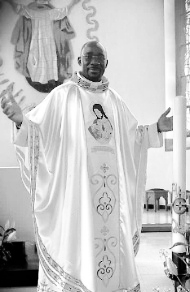
\includegraphics[scale=1.20]{../images/standing_daniel}
\end{wrapfigure}
C’est le sacrifice de soi.
Un renoncement radical, car suivre le Christ c’est renoncer à disposer de soi et à prendre l’initiative de sa vie.
Cela demande de tout miser sur celui que nous plaçons au centre de nos préoccupations et de nos pensées.
La véritable révolution de la vie chrétienne vient du renoncement, il conduit vers Dieu et vers les autres pour nous mettre humblement à leur service. 

\begin{flushright}
Bel été à toutes et à tous !!!
\textit{Père  Daniel  ETTÉ}
\end{flushright}

